\chapter{Dynamic time and state varying detection probability}
As stated in the Introduction, this work focuses on tracking objects in frame sequence using target tracking methods
and
object detection
and
segmentation algorithms. Object detectors, which were discussed in the previous section, are essential for getting
measurements
from an image.

Note, that in all target tracking algorithms for cluttered environments and targets
birth and dead possibilities, there is a parameter called the detection probability ($p_D$). As its name
suggests, this parameter expresses a probability that the target is detected in \linebreak a particular time. It is also commonly
used
as a
time- and state-independent scalar. The desired outcome is to enhance the performance of multi-target
algorithms in scenarios where the targets may be hidden by an obstacle and reduce impacts of a misdetection of a sensor.
Therefore, it
is appropriate to have a dynamic time- and state-varying detection probability.
\section{Problem definition}
\label{sec:mphd_problemDef}
In the practical part of this thesis, three different settings of object detection and segmentation can be found.
We choose Probability Hypothesis Density filter as a multi-target tracking algorithm, as it is a simpler
RFS-based method. PHD filter is computationally very effective in comparison with filters such as the CPHD or the
PMBM filter,
which may seem as a more appropriate option for this task. However, these more complicated filters have high
computational demands, which
are not adequate when used in video streams. Provided settings are:
\begin{enumerate}
  \item \textbf{S1: YOLO + PHD} -- Yolo itself can produce an object segmentation mask with lower accuracy, but with
  greater
  speed. This setting is suitable when using CPU only.
  \item \textbf{S2: YOLO + SAM + PHD} -- As SAM cannot annotate labels to objects, it requires another object detector
  before segmentation. In this setting, we use YOLO as an object detector and SAM for mask segmentation of detected
  objects. This procedure requires GPU for faster computation.
  \item \textbf{S3: Grounded SAM + PHD} -- Grounded SAM is the most universal approach, as it can detect objects based
  on a text input and uses SAM for segmentation. This setting also requires GPU for faster computation.
\end{enumerate}


\subsection{The modified GM-PHD filter}
To modify the GM-PHD filter for our use case, a few assumptions have to be introduced. These assumptions are very
similar to those of the PHD filter and the GM-PHD filter in Section \ref{sec:phdfilter} and \ref{sec:gmphdFilter}.
\begin{enumerate}
  \item Each target evolves and generates observations independently of each other. \label{as:mphd_1}
  \item Clutter is Poisson and independent of target-originated measurements. \label{as:mphd_2}
  \item The predicted multi-target RFS governed by $p_{k|k-1}$ is Poisson. \label{as:mphd_3}
  \item Each target follows a linear Gaussian dynamical model and the sensor has a linear \label{as:mphd_4}
  Gaussian measurement model, i.e.,
  \begin{align}
    f_{k|k-1}(x|\xi) &= \mathcal{N}(x; F_{k-1}\xi, Q_{k-1}),\\
    g_k(z|x) &= \mathcal{N}(z;H_kx, R_k),
  \end{align}
  where $\mathcal{N}(\cdot;\cdot,\cdot)$ is a Gaussian density, $Q_{k-1}$ is the process noise covariance, $H_k$ is the observation matrix and $R_k$ is the observation noise covariance.
  \item The survival probability is state-independent, i.e.,
  \begin{align}
    p_{S,k}(x) &= p_{S,k}.
  \end{align}
    \label{as:mphd_5}
  \item The detection probability is state-dependent, i.e.,
    \begin{align}
      p_{D,k}(x) &= 
      \begin{cases}
         p_{D,k} &\qquad \text{if detected for the first time,} \\
         p_{D,k}(x) &\qquad \text{otherwise.}
      \end{cases}
    \end{align}
    \label{as:mphd_6}
  \item The intensity of the birth RFS is a Gaussian mixture of the form
  \begin{align}
    \gamma_k(x) &= \sum_{i=1}^{J_{\gamma,k}}w_{\gamma,k}^{(i)} \mathcal{N}\left(x; m_{\gamma.k}^{(i)}, P_{\gamma,k}^{(i
    )}\right).
    \label{eq:mphd_intensity}
  \end{align}
  \label{as:mphd_7}
\end{enumerate}
Note, that the assumption \ref{as:mphd_1} may be questionable, as the states of each of the targets are often
dependently
evolving.
Imagine,
for example, a common traffic scenario. If one of the cars immediatelly stops, the following vehicles have to stop as
well. Meaning, they are affected by another target.
The assumption \ref{as:mphd_2} is reasonable, especially if we consider that the clutter rate should be very low in
our
scenarios.
The survival probability is state-independent as in the GM-PHD filter and should be set high, as the targets are
expected
to survive to the next time step.
The detection probability is state-dependent and equal to $p_{D,k}$, i.e., a predefined threshold, in situation when
the target is detected for the first time. Otherwise, if the target has evolved from the previous state $\xi$, the
detection probability is calculated according to Section \ref{sec:dynamic_pd}.
Assumption \ref{as:mphd_7} contains only intensity of the birth RFS, the spawn intensity RFS is left out.
Nevertheless, it still can be easily added to the assumption
and equations afterwards.

\subsubsection{The modified PHD recursions}
Let us assume a target state $x$ described by an intensity function $\nu(x)$. At time $k$, the prediction of the prior
intensity $\nu_{k-1}(x)$ is given by
\begin{equation}
  \nu_{k|k-1}(x) = \int p_{S,k}(\xi)\phi_{k|k-1}(x|\xi)\nu_{k-1}(\xi)d\xi + \nu_{\gamma,k}(x), \label{eq:mphdPrior}
\end{equation}
where $p_{S,k}(\cdot)$ is the probability of target survival, $\phi_{k|k-1}(\cdot|\cdot)$ is the target state transition density, and $\nu_{\gamma,k}(\cdot)$ denotes the prior PHD of the targets birth at time k.
The predicted intensity $\nu_{k|k-1}$ is then updated by the measurement set $Z_k$ given by sensors at time $k$ according to the Bayesian update
\begin{equation}
  \begin{aligned}
    \nu_k(x) &= [1 - p_{D,k}(x)]\nu_{k|k-1}(x) \\
    &+ \sum_{z \in Z_k}\frac{p_{D,k}(x) g_k(z|x) \nu_{k|k-1}(x)}{\kappa_k(z) + \int p_{D,k}(\xi) g_k(z|\xi) \nu_{k|
    k-1}(\xi)d\xi}, \label{eq:mphdPosterior}
  \end{aligned}
\end{equation}
where $g_k(\cdot|\cdot)$ is the likelihood function, $p_{D,k}(\cdot)$ is the probability of detection, and $\kappa_k(\cdot)$ is the clutter density.

\subsubsection{The modified GM-PHD recursion}
\label{sec:mGMPHDrec}
In the context of the linear Gaussian multiple-target model, the PHD recursion equations (\ref{eq:mphdPrior}) and (\ref{eq:mphdPosterior}) attain analytical solution \cite{VoMaPHD2006}.
Suppose that the posterior intensity at time $k-1$ is a Gaussian mixture of the form
\begin{equation}
  \label{eq:mphd_recursion_posterior}
  \begin{aligned}
    \nu(x) &= \sum_{i=1}^{J_{\gamma,k}} w_{\gamma,k}^{(i)}\mathcal{N}(x;m_{\gamma,k}^{(i)},P_{\gamma,k}^{(i)}).
  \end{aligned}
\end{equation}
The predicted intensity for time $k$ is also a Gaussian mixture of the form
\begin{equation}
  \label{eq:mphd_recursion_prior}
  \begin{aligned}
    \nu_{k|k-1}(x) &= \nu_{S,k|k-1}(x) + \gamma_k(x),
  \end{aligned}
\end{equation}
where $\gamma_k(x)$ is given in Formula (\ref{eq:mphd_intensity}). This yields
\begin{align}
  \nu_{S,k|k-1}(x) &= p_{S,k}\sum_{j=1}^{J_{k-1}}w_{k-1}^{(j)} \mathcal{N}(x;m_{S,k|k-1}^{(j)}, P_{S,k|k-1}^{(j)}) \label{eq:mphd_recursion_predict_intensity}, \\
  m_{S,k|k-1}^{(j)} &= F_{k-1}m_{k-1}^{(j)},  \label{eq:mphd_recursion_predict_m} \\
  P_{S,k|k-1}^{(j)} &= Q_{k-1} + F_{k-1}P_{k-1}^{(j)}F_{k-1}^T.  \label{eq:mphd_recursion_predict_P}
\end{align}
Thus the predicted intensity at the time $k$ is a Gaussian mixture
\begin{align}
  \nu_{k|k-1}(x) &= \sum_{i=1}^{J_{k|k-1}}w_{k|k-1}^{(i)} \mathcal{N}(x;m_{k|k-1}^{(i)}, P_{k|k-1}^{(i)}),  \label{eq:mphd_recursion_predict_intesity}
\end{align}
and the posterior intensity at time $k$ is also Gaussian mixture,
\begin{align}
  \nu_{k}(x) &= \sum_{i=1}^{J_{k|k-1}}[1-p_{D,k}^{(i)}(x)]w_{k|k-1}^{(i)} \mathcal{N}(x;m_{k|k-1}^{(i)}, P_{k|k-1}^{(
  i)})\nonumber \\
  &+ \sum_{z\in Z_k}\nu_{D,k}(x;z), \label{eq:mphd_recursion_update_intesity}
\end{align}
where
\begin{align}
  \nu_{D,k}(x;z) &= \sum_{j=1}^{J_{k|k-1}} w_k^{(j)}(z) \mathcal{N}(x;m_{k|k}^{(j)}(z),P_{k|k}^{(j)}), \label{eq:mphd_recursion_update_intesity_detect} \\
  w_k^{(j)}(z) &= \frac{p_{D,k}^{(j)}(x;z) w_{k|k-1}^{(j)} q_k^{(j)}(z) }{\kappa_k(z) + p_{D,k}^{(j)}(x;z) \sum_{l=1}^{J_{k|k-1}} w_{k|k-1}^{(l)} q_k^{(l)}(z)}, \label{eq:mphd_recursion_update_intesity_detect_w} \\
  m_{k|k}^{(j)}(z) &= m_{k|k-1}^{(j)} + K_k^{(j)}(z-H_k m_{k|k-1}^{(j)}), \label{eq:mphd_recursion_update_intesity_detect_m} \\
  P_{k|k}^{(j)}(z) &= [I - K_k^{(j)} H_k] P_{k|k-1}^{(j)},  \label{eq:mphd_recursion_update_intesity_detect_P} \\
  \kappa_{k}^{(j)}(z) &= P_{k}^{(j)} H_k^T(H_k P_{k|k-1}^{(j)} H_k^T + R_k)^{-1}. \label{eq
  :mphd_recursion_update_intesity_detect_K}
\end{align}
The dynamically estimated detection probability in \eqref{eq:mphd_recursion_update_intesity} follows from one of two
possible scenarios described in Section \ref{sec:dynamic_pd}.
\subsection{S1: YOLO + PHD}
It is possible to fine-tune YOLO model on personalised datasets to either improve the performance in the
detection of
pretrained classes, or to train the model for detecting other classes. With over 70 pretrained class instances, it is
not necessary to fine tune our YOLO model for the experiments in this work. The model also detects all class
instances it is trained for, that appear in a scene. For testing purposes, we filter only objects we want to detect
and get
measurements from. The YOLO itself is able to produce a segmentation mask in real-time, but with less
accuracy
and
precision. This is caused by a reduced image resolution which is $640x640$ pixels. To fit the YOLO output
to our
frame,
this output needs to be resized back to our desired frame size. This resizing causes some imperfections. However, the
precision
to pixel level is not always necessary in our scenarios, thus this setting is, in most cases, sufficient
enough. The advantage of this approach is that it runs quickly enough with CPU only. The example of
object segmentation YOLO model is shown in the Figure \ref{fig:yolo_seg}.
\begin{figure}[h]
  \centering
  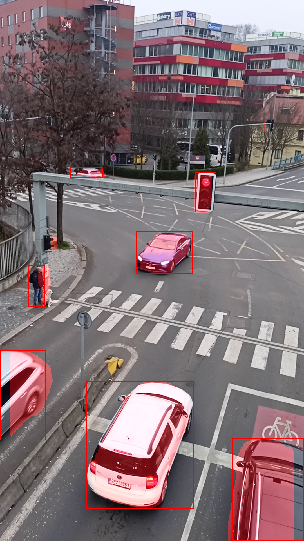
\includegraphics[width=0.35\linewidth]{text/chapter_04/imgs/YOLO_screenshot_2}
  \caption{YOLO segmentation example. This picture shows all detected objects the YOLO model is trained for and also
  the segmented objects' masks. These masks are imperfect, but often sufficient enough. (Kartouzská street, Prague)}
  \label{fig:yolo_seg}
\end{figure}

\subsection{S2: YOLO + SAM + PHD}
The SAM model architecture in \cite{SAM2023} is prepared to first process a text input and then segment objects based
on the
input. However, this feature is not available yet in the original implementation, and, for our purposes, we need an
object
detector before the segmentation process can be performed. The SAM model is able to segment a desired object based on
one
of two provided
inputs with high precision and accuracy. The first possible input is a bounding box around the required object, which
can be provided by an output of the YOLO model. The second option is to provide a rough center point of an object, which
can also be the center of a bounding box provided by the YOLO model.

However, for our purposes, it is not recommended
to use the combination of both inputs, as SAM is able to produce multiple masks for an object. For example, if we
denote that we want to segment a whole person by a bounding box, one of the output masks can be just his jacket, as it
makes a
valid segmentation mask. Combining these two inputs can, therefore, produce this undesirable output. Another
example of
such
behavior
is shown in the Figure \ref{fig:sam_examples}
\begin{figure}[htbp]
  \centering
  \begin{subfigure}[h]{0.48\textwidth}
    \centering
    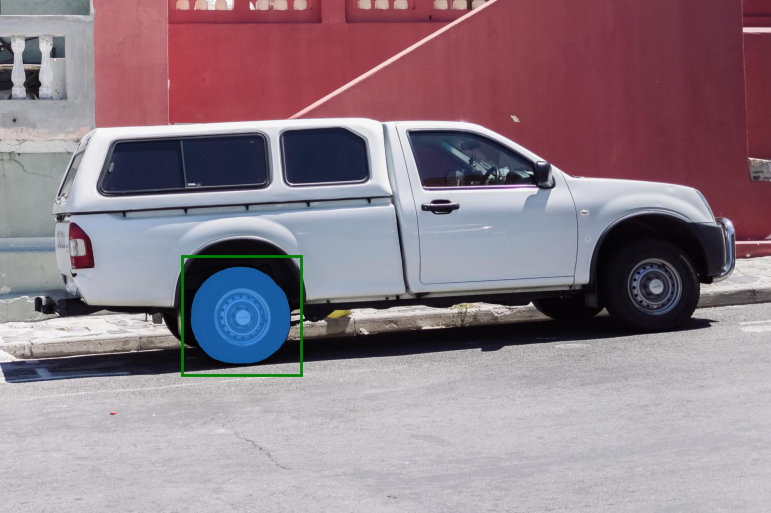
\includegraphics[width=\textwidth]{text/chapter_04/imgs/SAM_box}
    \caption{By defining an object by a bounding box, SAM is able to make a segmented masks of this object and choose
    the most probable one.}
    \label{fig:sam_box}
  \end{subfigure}
  \hfill
  \begin{subfigure}[h]{0.48\textwidth}
    \centering
    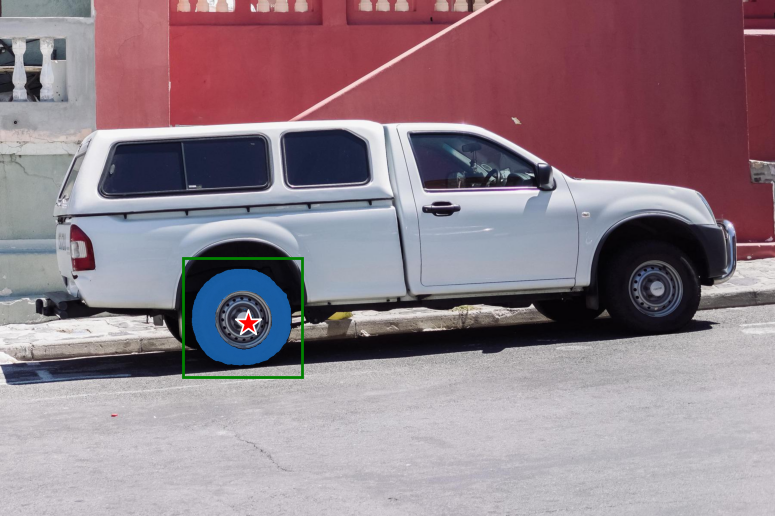
\includegraphics[width=\textwidth]{text/chapter_04/imgs/SAM_box_point}
    \caption{If we use a bounding box together with a point, we receive a different result. Here, just the trucks's
    tire, instead of the entire wheel, is selected.}
    \label{fig:sam_boxPoint}
  \end{subfigure}
  \caption{Comparison of using only a bounding box vs combination of a bounding box and a point as an input for SAM.}
  \label{fig:sam_examples}
\end{figure}

The combination of the SAM model with an object detector can segment an object with high precision and accuracy.
The cooperation of these two models is demonstrated in Figure \ref{fig:yolo_sam_seg}.
\begin{figure}[h!t]
  \centering
  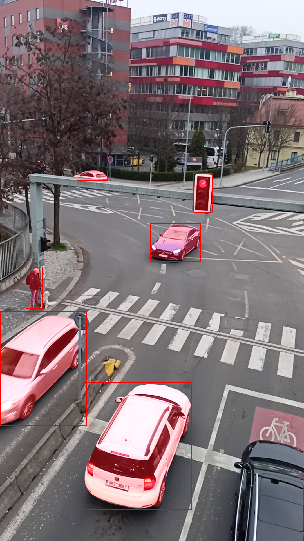
\includegraphics[width=0.35\linewidth]{text/chapter_04/imgs/YOLO_SAM_02}
  \caption{The cooperation of YOLO and SAM models. The YOLO provides bounding boxes of objects, which are inputs to
  SAM. The SAM model then makes segmented masks of these objects. (Kartouzská street, Prague)}
  \label{fig:yolo_sam_seg}
\end{figure}

\subsection{S3: Grounded SAM + PHD}
Grounding DINO is an object detector that denotes objects in an image, based on a given text prompt. This feature
allows us to potentially track all the required objects without the need to fine tune every class instance to a model.
Moreover, this
model is able to mark objects based on an ambiguous text input. Despite this universality,
in cases where the
model is not confident enough that the desired object appears in a scene, different results can be received with
the same input every time the model is executed. This brings uncertainty in situations with ambiguous text inputs
and we should be aware of it in practical scenarios.

For a segmentation task, Grounding DINO's output serves as an input to the SAM model, as it produces bounding boxes
of the
detected objects.
SAM uses these bounding boxes to segment objects and creates segmentation binary masks. The cooperation of these models is demonstrated in Figure \ref{fig:GroundedSAM}.

\begin{figure}[h]
  \centering
  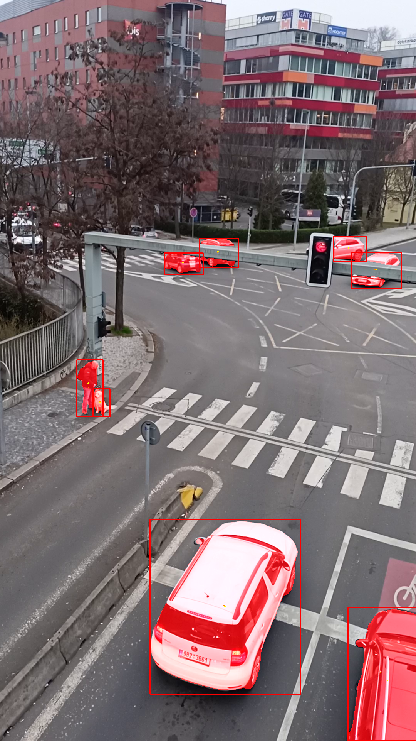
\includegraphics[width=0.35\linewidth]{text/chapter_04/imgs/DINO_example}
  \caption{The result of the Grounded SAM model. Grounding DINO marks objects with bounding boxes and SAM segments
  objects inside these bboxes. Marked objects are founded by Grounding DINO with text input \textit{person, car}. (Kartouzská street, Prague)}
  \label{fig:GroundedSAM}
\end{figure}



\section{Dynamic detection probability in video data}
\label{sec:dynamic_pd}
To model the dynamic state- and time-dependent detection probability $p_{D,k}(x)$, we propose to base the current
point estimate of $p_{D}(x)$ at time $k$ on the similarity of the subsequent frame properties,

  \begin{align}
    p_{D,k}(x) &= \frac{\sum_{\sigma_j \in S_{sim}} \sum_{i=1}^{|H|}
      \sigma_j\left[h_i\left(M(x; k|k-1) \!\circ\! D_k\right),
        h_i\left(M(x; k-1) \!\circ\! D_k\right)\right]}{\|S_c\| \cdot \|H\|}, \label{eq:similarity}
  \end{align}
where $D_k$ is the frame in the given color spectrum, $h_i(\cdot)$ is a color histogram made from given color spectrum, $A\circ B$ is the Hadamard product, $M(\cdot, \cdot)$ is the object binary mask, and $\sigma_j[\cdot, \cdot]$ is
the given similarity of two vectors. $\|\cdot\|$ denotes the set size. The whole
fraction is, in fact, the mean value across all color spectra and similarity functions.

There are many color spectra to consider, each providing certain benefits and downsides. The list of color spectra used
in this work is as follows.
\begin{itemize}
  \item \textbf{RGB} -- The RGB (Red, Green, Blue) color model is ubiquitous in electronic displays, digital cameras, and computer graphics. It defines colors by their intensities of red, green, and blue components. One of its
  primary advantages lies in its widespread use and an intuitive representation for additive color mixing. However,
  RGB lacks direct perceptual relevance to human vision, as it does not inherently represent attributes like brightness
  or hue.
  \item \textbf{XYZ} -- In contrast, the XYZ color space, established by the International Commission on Illumination
  (CIE), serves as a standard for quantifying colors in scientific and industrial applications. Even though it offers a
  device-independent color representation and facilitates color matching and conversion, it is not as perceptually
  intuitive and can be complex to work with practically.
  \item \textbf{HSV} -- HSV (Hue, Saturation, Value) is favored in graphics software and image editing for its
  intuitive representation of color. It aligns better with human perception compared to RGB, allowing independent
  adjustment of hue, saturation, and brightness. It lacks the widespread hardware and software support enjoyed by RGB
 and may not be as straightforward for certain color manipulation
  tasks.
  \item \textbf{LAB} -- LAB (CIELAB color space), another CIE-defined model. Unlike
  XYZ, it aims for perceptual uniformity. Widely used in color correction, image editing, and color management, LAB
  offers uniform changes in perceived color with uniform changes in LAB values. Despite its perceptual accuracy, it
  can be complex to comprehend and lacks universal software and hardware support compared to simpler models like RGB
  or HSV.
  \item \textbf{HLS} --  HLS (Hue, Lightness, Saturation) finds its place in computer graphics and image editing
  applications. Similar to HSV but with lightness instead of value, HLS provides an intuitive representation for
  color adjustment tasks. Unfortunatelly, its support may not be as widespread as RGB or HSV, and it may lack the
  perceptual accuracy of LAB in certain color correction scenarios.
\end{itemize}

We apply a range of similarity functions, each with its unique advantages and limitations. These functions include cosine similarity, intersection, and correlation.
\begin{itemize}
  \item \textbf{Cosine similarity} -- Cosine similarity, a widely used metric, determines the cosine of the angle
  between two vectors in a multi-dimensional space. It is insensitive to vector magnitudes, focusing more on their
  orientation, which proves valuable when the absolute magnitude of vectors is less crucial than their relative
  orientations. However, cosine similarity does not take into account the distribution of data points. Cosine
  similarity is defined as
  \begin{align}
    S_{cos} [A,B] &= \frac{A\cdot B}{\|A\|\|B\|} = \frac{\sum_{i=1}^nA_iB_i}{\sqrt{\sum_{i=1}^nA_i^2} \cdot \sqrt{\sum_{i
    =1}^n B_i^2}},
  \end{align}
  where the sums run over all elements of the arguments.
  \item \textbf{Intersection} -- Intersection similarity, on the other hand, calculates the overlap between two sets. This metric is commonly employed in applications like document retrieval and collaborative filtering. Its
  simplicity and intuitiveness make it ideal for comparing binary data or sets, where the presence or absence of
  elements is more significant than their values. Additionally, it treats all elements equally, disregarding their
  magnitudes, which can be a limitation in certain contexts. The intersection is formulated
    \begin{align}
      S_{inter}[A,B] &= \frac{\sum_{i=1}^{\|A\|} \min(A_i, B_i) }{\sum_{i=1}^{\|B\|} B_i},
    \end{align}
    where $\|\cdot\|$ denotes the set size.
  \item \textbf{Pearson correlation coefficient} -- Correlation measures the linear relationship between two
  variables and is frequently used in statistics, finance, and signal processing. It captures both the strength and
  direction of the relationship between variables, making it valuable for identifying patterns and dependencies in
  data. Moreover, correlation assumes a linear relationship between variables, which may not always hold true, and it
  is susceptible to outliers and non-linear relationships, potentially  affecting its reliability in certain scenarios. In this work, we calculate the correlation between corresponding elements in sets $A, B$ as
    \begin{align}
      S_{corr}[A,B] &= \frac{\operatorname{cov}(A,B)}{\sigma_A \sigma_B},
    \end{align}
    where $\operatorname{cov}$ is the covariance and $\sigma_{(\cdot)}$ is the standard deviation,
\end{itemize}

For simplicity, let us denote the fraction in \eqref{eq:similarity} as $S_c$. This value represents the "average"
similarity across all used color spectra and similarity functions.

As mentioned in Section \ref{sec:mGMPHDrec}, the dynamically estimated detection probability in \eqref{eq:mphd_recursion_update_intesity} follows from one of two possible scenarios. First, there is no current measurement at
time $k$, hence the current mask results from its predicted position,
\begin{align}
  \label{eq:mphd_recursion_update_intesity_misdetect_pd}
  p_{D,k}^{(i)}(x) &=
  \begin{cases}
     S_c^{(i)}\left[h(M_{k|k-1}^{(i)}(x) \circ D_k), h_{0,k}^{(i)}\right] &\text{if $h_{0,k}^{(i)}$ exists,} \\
     p_{D,k}^{(i)} \quad& \text{otherwise,}
  \end{cases}
\end{align}
and where the histogram from the last detection $h_{0,k}^{(i)} \equiv  h_{0,k-1}^{(i)}$ is used in the first scenario. A user-preset value $p_{D,k}^{(i)}$ is used for targets undetected so far. The mask is obtained via
\begin{align}
  \label{eq:mphd_recursion_update_intesity_misdetect_M_shifted}
  M_{k|k-1}^{(i)}(x) &=
  \begin{cases}
    \!M_{k-1}^{(i)}(x)[m-v_x, n-v_y] &\text{if $m\geq v_x, n\geq v_y$,} \\
    \mathbf{0} \quad &\text{otherwise,}
  \end{cases}
\end{align}
where $m, n$ are indices of the binary mask $M$ and $v_x, v_y$ are x- and y-direction velocities of the target. $\mathbf{0}$ is a zero vector of the same size as the mask. The second scenario takes the current measurement $z$ into account. The detection probability is modified according to
\begin{align}
  p_{D,k}^{(j)}(x;z) &= S_c\left[h(M_{k}^{(j)}(z) \circ D_k), h_{0,k}^{(j)}\right], \label{eq:mphd_recursion_update_intesity_misdetect_z_pd}
\end{align}
where $h_{0,k}^{(j)}$ is the histogram resulting from the last detection,
\begin{equation}
  \label{eq:mphd_recursion_update_intesity_misdetect_Hist}
  h_{0,k}^{(j)} =
  \begin{cases}
    h(M_{k-1}^{(j)}(z) \circ D_{k-1}) &\text{if } h(M_{k-1}^{(j)}(z)) \text{ exists,} \\
    % h(M_{k|k-1}^{(j)}(x) \circ D_{k_0}) &\text{otherwise,} \\
    h_{0,k-1} &\text{otherwise.}
  \end{cases}
\end{equation}
The histogram $h(M_{k-1}^{(j)}(z) \circ D_{k-1})$ stands for the previously detected target, and $h_{0,k-1}$ is the histogram from the time step when the target was detected the last time.



\section{Modified pruning for GM-PHD filter}
As the PHD filter propagates the posterior intensity, the number of potential hypotheses exponentially increases.
This leads to an enormous increase in memory and computational demands. Pruning techniques become indispensable in
mitigating this computational load by selectively discarding less likely hypotheses, allowing for a more focused and
efficient tracking process. These pruning mechanisms, guided by predefined thresholds or heuristics, ensure that the
computational resources are allocated judiciously, striking a balance between accuracy and computational efficiency in multi-target tracking applications.

Recall that sensors in our work are represented by cameras. Naturally, the detecting algorithms are unable to
recognize an object hidden by an obstacle. These obstacles may differ not only in size but also in color. In
situations where the color of an obstacle closely matches the surrounding scene, the likelihood of detection remains
sufficiently high, increasing the risk that the target may not survive even though it is only hidden. In order to suppress this phenomenon, we introduce a method for modified pruning along with the standard pruning and merging techniques \cite{VoMaPHD2006}.

The most deployed generic method for pruning consists of removing targets with weights below some predefined threshold. Nonetheless, as mentioned before, targets with some history may only be hidden, and it is not desired to remove these targets from the scene. To overcome this issue, we assign each target a tag that represents the state in which the target is likely to occur,
\begin{equation}
  S = \{\text{detected, hidden, dead}\}.
  \notag
\end{equation}
This tag is modeled by a discrete-time Markov chain with the transition matrix
\begin{align}
  \label{eq:mphd_transition_matrix}
  P &= \begin{bmatrix}
         p_{D,k} & 1-p_{D,k} & 0 \\
         p_{D,k} & (1-p_{H,k}^{T_H}) \cdot (1-p_{D,k}) & p_{H,k}^{T_H} \cdot (1- p_{D,k}) \\
         p_{D,k} & (1-p_{H,k}^{T_H}) \cdot (1-p_{D,k}) & p_{H,k}^{T_H} \cdot (1- p_{D,k})
  \end{bmatrix},
\end{align}
where $p_{D,k}$ is a generic detection probability, and $T_H$ is an exponent for controlling probabilities that is
set higher in scenarios, where the target color mask is similar to the color mask of the obstacle, or may be set
lower otherwise. $p_{H,k}$ is the probability that the target is removed. This probability is the result of \eqref{eq:mphd_recursion_update_intesity_misdetect_pH}, where the bounding boxes of the object detector are used.
If we denote by $B_{P,k}^{(j)}$ the bounding box predicted $T_c$ steps ahead and by $B_{S,k}^{(j)}$ the bounding box of the last step $k$ when the object was detected, then
\begin{align}
  B_{P,k}^{(j)} &= B_{P,k-1}^{(j)} + n_k^{(j)}\cdot [v_{x,{k}}^{(j)}, v_{y,{k}}^{(j)}, _{x,{k}}^{(j)}, v_{y,{k}}^{(j)}], \label{eq:mphd_bbox_shift}\\
  B_{S,k}^{(j)} &= B_{S,k-1}^{(j)}, \\
  p_{H,k} &= S_c\left[D_k(B_{P,k}^{(j)}), D_k(B_{S,k}^{(j)})\right], \label{eq:mphd_recursion_update_intesity_misdetect_pH}
\end{align}
where
\begin{align}
  \label{eq:mphd_recursion_update_intesity_misdetect_T_move}
  n_k^{(j)} &=
  \begin{cases}
    T_c \quad & \text{if } k\text{ } mod \text{ }T_c = 0,  \\
    0 \quad & \text{otherwise.}
  \end{cases}
\end{align}
$D_k(\cdot)$ is a part of a frame within the bounding box given by $B(\cdot)$. With this approach, when a target is most likely in the \textit{hidden} state, the pruning threshold is heuristically lowered to prevent the target removal.

In summary, first we define a birth place in a scene. We call this birth place a spawn point (SP). It is possible to
define more spawn points in a scene, depending on the situation. If a target appears at this spawn point, it is
initialized, and since it is the first time the target has been seen, the detection probability is a predefined
constant. In the
next time step, suppose that the target is detected and there is one measurement (originating from this target) in the
validation region. Due to the GM-PHD recursion, two new targets arise from the previous target with the state $\xi$.
One originates from
the misdetection possibility and one from the measurement. As
we first predict the target's position and covariance
matrix, we move the target's mask detected at time $k-1$ to $k$ by its velocity (in case of the CVM model). Then the
predicted mask color properties are compared to the mask made from the new measurement from time $k$. If nothing
unpredictable happens, both masks should occur on a very similar position, thus the color masks' properties should be
very similar. In such case, the detection probability is very likely to be high, lowering the weight of the
misdetection-born target. As the weight is small, the target is likely to be removed during the pruning step.

If the previously detected target is hidden behind an obstacle and the object detector does not provide any
measurement, only misdetection-born target arises. In such case, the mask from the time when the target was lastly
detected is compared to the predicted mask that now also contains the obstacle's color properties. Due to using
a camera as
a sensor, frames at high frame rate are produced. To prevent the loss of significant information, lowering the fps to a minimal rate is not desirable. We lower the fps to 10-30 fps to enhance the dynamics of the scene. However, in a such short time
period, the target, e.g. a car, does not move enough. The predicted mask then intersects with the lastly
detected target's mask by a considerably huge amount. That is why we define \linebreak a probability of the target to be hidden (\textit{hidden probability}, $p_{H,k}$) and modify
the pruning of components. As the masks are likely to intersect, the detection probability is likely to be high in
the first couple of frames, where the target is hidden. It is essential for the target to survive through this time
period. The hidden probability is based on the color properties of bounding boxes from the time the target was lastly
detected
and from the bounding box that is moved $T_c$ time steps ahead in the direction of the target's velocity. The moved
bounding box reveals the color properties of the obstacle, that are likely to be different from those assigned to the
target
when it was lastly detected. Then, the hidden probability should be low and the target's state should be in a hidden
state,
based on \eqref{eq:mphd_transition_matrix}, therefore the pruning threshold is lowered. After the target overtakes the
obstacle,
it should appear in a scene and be detected again. If it does not and the color properties of a scene given by the
moving
bounding box differ from the ones captured when the target was lastly detected, the hidden probability is high and the
target is
in \linebreak a dead state. The pruning threshold is not lowered and the detection probability is low, so the target is removed
during the pruning step.
\section{Merging in GM-PHD filter with dynamic detection probability}
Another way to lower the computational demands and to potentially increase the robustness of a filter is through
merging of the
targets that appear in the same neighbourhood. This procedure is especially useful in situations when many measurements
occur in \linebreak a validation region of a target. If at least some of these measurements originate from clutter, the target
count increases rapidly due to the
GM-PHD recursion, increasing the computational requirements. To prevent this issue,
the target merging technique is \linebreak necessary.
In the GM-PHD filter, each target carries three variables: the target's weight $w$, mean $m$ and a covariance matrix $P$.
Merging these values of multiple filters is straightforward and is described in \cite{VoMaPHD2006} and Section \ref{sec:phd_pruning_and_merging}. However, in our modified GM-PHD filter, each target also holds these information:
\begin{itemize}
  \item \textbf{Current bounding box position:} The bbox in $xyxy$ format determines current position of an object.
  This bbox is determined by a bbox given by a measurement $z$ in the current time step $k$ in an update step. The
  target's
  bbox is shifted in the prediction step in \eqref{eq:mphd_bbox_shift}, thus the target must have been initialized in
  the
  past in order to have the current bbox.
  \item \textbf{Current mask:} The current binary mask is given by a measurement $z$ in the current time step $k$ in
  the update
  step. In order to inialize current mask, it must have been initialized by a measurement in
  the past. The mask is shifted according to \eqref{eq:mphd_recursion_update_intesity_misdetect_M_shifted}.
  \item \textbf{Object Stats:} Every new target born in the update step of the GM-PHD filter by a
  measurement $z$ from a target with a previous state $\xi$, contains a data structure \textit{Object Stats}. This
  structure is composed of many variables determining the target's history. These variable arise in the update step from
  a measurement and are useful for calculating the dynamic detection probability in Equations
  \eqref{eq:mphd_recursion_update_intesity_misdetect_pd} - \eqref{eq:mphd_recursion_update_intesity_misdetect_pH}.
      \begin{itemize}
        \item \textbf{Bounding box position:} This variable in \textit{Object stats} represents a bounding box from the time
        the target was lastly detected. To calculate $p_{H,k}$ in
        \eqref{eq:mphd_recursion_update_intesity_misdetect_pH}, this and the current bbox are compared.
        \item \textbf{Mask:} This variable represents the target's mask from the time the target was lastly detected. In \eqref{eq:mphd_recursion_update_intesity_misdetect_pd} and \eqref{eq:mphd_recursion_update_intesity_misdetect_z_pd} this mask is compared to the current mask
        resulting from the prediction step of a target with the previous state $\xi$.
        \item \textbf{Frame:} To compare the color histograms in \eqref{eq:mphd_recursion_update_intesity_misdetect_pd}
        and \eqref{eq:mphd_recursion_update_intesity_misdetect_z_pd}, each target contains a frame from the time $k$
        in which
        it was born.
        \item \textbf{Time stamp:} This is a variable to save the time $k$ the target was born.
      \end{itemize}
  \item Data structure \textbf{Markov Chain:} This data structure determines the target's state. As the
  distribution determined by a transition matrix in \eqref{eq:mphd_transition_matrix} is not stationary, it is necessary
  to calculate the resulting distribution in every time step.
      \begin{itemize}
        \item \textbf{Initial distribution:} To get the target's state, an initial distribution needs to be defined
        first.
        \item \textbf{Result matrix:} The result matrix is an ongoing outcome of a previous result matrix and a
        transition
        matrix, i.e, the result matrix $R_k = R_{k-1} P^{k-k_0}$, where $k_0$ is the time the target was born,
        $R_0 = I_3$ and $I_n$ is the identity matrix of the shape $n\times n$.
      \end{itemize}
\end{itemize}

The merging procedure of the previous information is inspired by the original GM-PHD merging procedure in
\cite{VoMaPHD2006}.

The current bounding box merging is straightforward as $(x_1,y_1)$ and $(x_2,y_2)$ coordinates defining the bbox are
averaged using the targets' weight. Let us define a set $L$, which represents a subset of targets to merge into a single
target. Then a resulting target's bbox
\begin{align}
  \tilde{B}_k^{(l)} &= \frac{\sum_{i \in L} B_k^{(i)} \cdot w_k^{(i)}}{\sum_{i \in L}{w_k^{(i)}}},
\end{align}
where $w_k^{(i)}$, is the weight of a target $i$ is the weighted mean of targets in subset $L$. The same procedure is
applied to the bounding box in \textit{Object Stats}, i.e., the previous bbox.

The merging of masks is slightly complicated, as we merge targets' masks into \linebreak a single "average" mask. First, binary
masks of targets in the subset $L$ are converted into \textit{float} data type, then multiplied with targets' weight
and
divided by the sum of these weights. To get the resulting binary mask, each element of mask
\begin{align}
  \tilde{M}_k^{(l)} &= \frac{\sum_{i \in L} M_k^{(i)} \cdot w_k^{(i)}}{\sum_{i \in L}{w_k^{(i)}}}
\end{align}
is rounded either to zero or one and the mask is converted to the binary data type.

We have not experimented with complicated merging of frames and time stamps, only argument maxima is used for both
values, i.e,
\begin{align}
  \tilde{t}_k^{(l)} &= \max_{i \in L} t_k^{(i)}, \\
  \tilde{D}_k^{(l)} &= D_k^{(\tilde{t}_k^{(l)})}.
\end{align}

As the initial distribution is the same for every target, the resulting merged target's initial distribution is only a
copy of any target in $L$.

The result matrix merging procedure is similar to the bounding box distribution. The resulting matrix
\begin{align}
  \tilde{N}_k^{(l)} &= \frac{\sum_{i \in L} N_k^{(i)} \cdot w_k^{(i)}}{\sum_{i \in L}{w_k^{(i)}}}
\end{align}
is the "average" result matrix of targets in subset $L$.

The pseudo-code algorithm of modified pruning in GM-PHD filter is shown in Algorithm \ref{alg:mphd_merging}.
\begin{algorithm}
  \caption{Pseudo-algorithm for pruning in the GM-PHD filter}
  \begin{algorithmic}[1]
    \Require{$\{w_{k}^{(i)}, m_{k}^{(i)},P_{k}^{(i)}, B_{k}^{(i)}, M_{k}^{(i)}, B_{OS,k}^{(i)}, M_{OS,k}^{(i)}, t_{OS
    ,k}^{(i)}, D_{k}^{(i)}, G_{OS,k}^{(i)}, N_{OS,k}^{(i)}\}_{i=
    1}^{J_{k}}$, a
    truncation
    threshold T, a
    merging
    threshold U and a maximum number of allowed Gaussian terms $J_{max}$. Set $l=0,$ and
      $I = \{ i=1,\dots, J_k | w_k^{(i)} > T\}$.}
    \Procedure{Merging of targets}{}
      \While{$I \neq \emptyset$}
        \State $l:= l+1$
        \State $j:= \text{argmax}_{i \in I} w_k{(i)},$
        \State $L:= \left\{ i \in I | (m_k^{(i)} - m_k^{(j)})^T (P_k{(i)})^{-1} (m_k^{(i)} - m_k^{(j)}) \leq U \right\},$
        \State $\tilde{w}_k^{(l)} = \sum_{i \in L} w_k^{(i)}$,
        \State $\tilde{m}_k^{(l)} = \frac{1}{\tilde{w}_k^{(l)}} \sum_{i \in L} w_k{(i)} x_k^{(i)},$
        \State $\tilde{P}_k^{(l)} = \frac{1}{\tilde{w}_k^{(l)}} \sum_{i \in L} w_k^{(i)} (P_k^{(i)} + (m_k^{(l)} - m _k^{(i)}) (m_k^{(l)} - m _k^{(i)})^T,$
        \State $\tilde{B}_k^{(l)} = \frac{1}{\tilde{w}_k^{(l)}} \sum_{i \in L} B_k^{(i)} * w_k^{(i)}$
        \State $\tilde{M}_k^{(l)} = round(\frac{1}{\tilde{w}_k^{(l)}} \sum_{i \in L} M_k^{(i)} * w_k^{(i)})$
        \State $\tilde{B}_{OS,k}^{(l)} = \frac{1}{\tilde{w}_k^{(l)}} \sum_{i \in L} B_{OS,k}^{(i)} * w_k^{(i)}$ \Comment{OS stands for Object Stats}
        \State $\tilde{M}_{OS,k}^{(l)} = round(\frac{1}{\tilde{w}_k^{(l)}} \sum_{i \in L} M_{OS,k}^{(i)} * w_k^{(i)})$
        \State $\tilde{t}_{OS,k}^{(l)} = max_{i \in L} t_{OS,k}^{(i)}$
        \State $\tilde{D}_{OS,k}^{(l)} = D_k^{(\tilde{t}_{OS,k}^{(l)})}$
        \State $\tilde{G}_{OS,k}^{(l)} = {G}_{OS,k}^{(j)}$ \Comment{Initial distribution of Markov process}
        \State $\tilde{N}_{OS,k}^{(l)} = \frac{1}{\tilde{w}_k^{(l)}} \sum_{i \in L} N_{OS,k}^{(i)} * w_k^{(i)}$
        \State $I:= I/L.$
      \EndWhile
    \EndProcedure
    \State
    \State If $l > J_{max}$ then replace $\{ \tilde{w}_k^{(i)}, \tilde{m}_k^{(i)}, \tilde{P}_k^{(i)}, \tilde{B}_k^{(i
    )}, \tilde{M}_k^{(i)}, \tilde{B}_{OS,k}^{(i)}, \tilde{M}_{OS,k}^{(i)}, \tilde{t}_{OS,k}^{(i)}, \tilde{D}_{OS,k}^{(i)}, \tilde{G}_{OS,k}^{(i)}, \tilde{N}_{OS,k}^{(i)} \}_{i=1}^l$ by
    those of the $J_{max}$ Gaussians with largest weights.
    \State
    \State Output: $\{ \tilde{w}_k^{(i)}, \tilde{m}_k^{(i)}, \tilde{P}_k^{(i)}, \tilde{B}_k^{(i
    )}, \tilde{M}_k^{(i)}, \tilde{B}_{OS,k}^{(i)}, \tilde{M}_{OS,k}^{(i)}, \tilde{t}_{OS,k}^{(i)}, \tilde{D}_{OS,k}^{(i)}, \tilde{G}_{OS,k}^{(i)}, \tilde{N}_{OS,k}^{(i)} \}_{i=1}^l$ as pruned Gaussian components.

  \end{algorithmic}
  \label{alg:mphd_merging}
\end{algorithm}
